\documentclass[margin=2mm]{standalone}

\usepackage{tikz}
\usetikzlibrary{positioning,calc}

\begin{document}
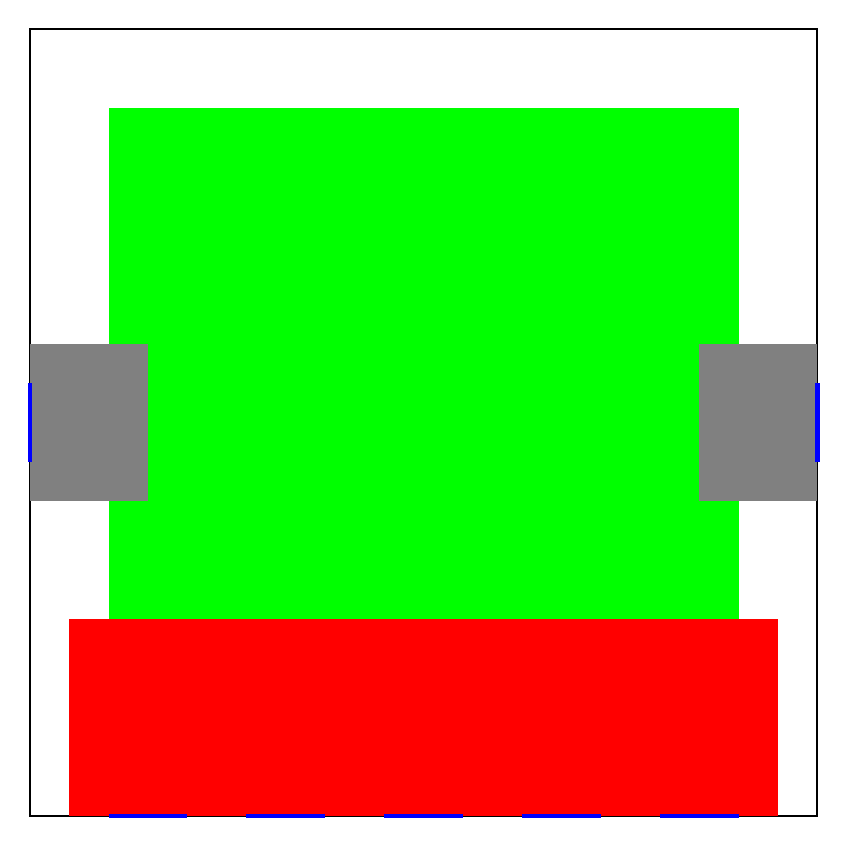
\begin{tikzpicture}
    \draw[thick] (0,0) rectangle ++(10,10);

    \fill[green] (1,1) rectangle ++(8,8);

    \fill[red] (0.5,0) rectangle ++(9,2.5);
    \fill[gray] (0,4) rectangle ++(1.5,2);
    \fill[gray] (10,4) rectangle ++(-1.5,2);

    \foreach \x in {0,1,2,3,4} {
        \draw[ultra thick,blue] (1.75*\x+1,0) -- ++(1,0);
    }
    \draw[ultra thick,blue] (0,4.5) -- ++(0,1);
    \draw[ultra thick,blue] (10,4.5) -- ++(0,1);




\end{tikzpicture}
\end{document}